\documentclass[../sherrill-Mix_thesis.tex]{subfiles}
\begin{document}
\chapter{Conclusions and future directions}
\graphicspath{{im/}{conclusion/im/}}

In this dissertation, we described studies to characterize the nature of HIV-1 latency, characterize expression and alternative splicing and host cell response to infection and develop alternative methods for detection of infection and quantification of viral loads.


\section{Latency and integration location}

	In Chapter \ref{chapLatency}, we showed that the chromosomal location of integration affects proviral latency but the mechanisms appear to differ between cell culture models. This suggests that either some cell culture models do not accurately reflect latency in patients or that there are diverse subsets of cells with differing mechanisms of latency within patients.

	Cell culture models are currently used to screen potentially therapeutic compounds. If some cell culture models are not representative of \textit{in vivo} conditions then potential treatments may be discarded or marked for development erroneously. Further comparisons between additional cell culture models and additional replicates of existing models might allow discrimination between batch/lab effects and reveal patterns in model behavior. Comparison with cells extracted from patients or infected lab animals might offer a gold standard comparison although it is difficult to obtain large amounts of cells and difficult to distinguish defective provirus from latent provirus in such populations. %Perhaps cell sorting for a marker of viral activity, applying a strong inducing agent and sorting again for newly expressed virus.

	Various treatments are now being considered for the reactivation of latent provirus \citep{Spina2013}. To further understand the mechanisms of these treatments, it would be interesting to compare latent provirus induced by a treatment to latent viable provirus remaining uninduced. Repeated cell sorting and integration site sequencing might provide insight on mechanism. For example, one could first sort out cells with active provirus, then treat with the potential latency modulator and sort out cells with newly active provirus and then treat with a strong inducer or alternative stimuli and sort out cell with these newly activated provirus. This would give two subsets of cells where latent viruses had been activated by treatment and cells which were not activated by treatment but still inducible. Synergies between treatments could be assessed and the location of integration sites could be determined and used to locate patterns of genomic features correlated with induction for each treatment.

	Current efforts at ``shock and kill'' therapy focus on histone deacetylase inhibitors. If there are diverse mechanisms of latency within patients then much of the latent reservoir may remain unactivated by single target therapies.  A recent study of potential latency modulators found that no single cell culture model reliably predicted in various cell culture models revealed little agreement \citep{Spina2013} [[work]][[also little effect?]]. Clinical trials with these therapies have shown some small increases in viral RNA \citep{Archin2012} but little decrease in the latent reservoir of HIV \citep{Archin2014,Spivak2014}. majority of latent provirus not reactivated by SAHA \citep{Cillo2014}. These results since 10,000-fold or more reductions of the latent reservoir are likely necessary for a functional cure for HIV \citep{Hill2014}.

%http://journals.plos.org/plospathogens/article?id=10.1371/journal.ppat.1003834


A common theme was that cell lines and \textit{in vitro} models of these replication steps often disagree with each other and with primary cell data. 


Comparison among labs and cell types/viruses at same time. Standardize.

Non polyadenylated RNA. Strand specific sequencing. Longer reads and longer fragments.

\section{HIV-1 alternative splicing}
Further clarification using more detailed sequencing in more time points, cell types and strains of HIV-1 and other lentiviruses rema

PacBio was bad. Figure? Do better

In addition an important subset of HIV are the founder viruses transmitted between hosts \citep{Keele2008,Salazar-Gonzalez2009}. These viruses are not well studied and perhaps their splicing and gene expression differ from the rest of the viral swarm of late-term patients.

\section{Host expression during HIV infection}
Localization nucleus vs cytoplasm

Cell types, macrophages

Infection, sorting

Cell lines bad

Endogenous retrovirus

\section{LAMP PCR and lab-on-a-chip}
		In Chapter \ref{chapLamp}, we report a loop mediated isothermal amplification system using primers optimized to to detect most subtypes of HIV-1. An alternative to a single broadly targeted primer set would be to design separate primer sets targeted specifically to each subtype so that a positive amplification would then be able to discriminate viral subtype. Different viral subtypes can have different rates of disease progression \citep{Kanki1999,Kaleebu2002,Baeten2007,Kiwanuka2008}, transmission dynamics \citep{Renjifo2004,John-Stewart2005,Huang2007b} and response to treatment \citep{Snoeck2006,Easterbrook2010,Scherrer2011}. Simple low-cost devices with multiple reactions chambers could be used to both identify viral subtype and estimate viral load \citep{Liu2014a,Mauk2015} and allow modified treatment decisions.
		
		A LAMP chip with subtype-specific primers would also allow the detection of some superinfections. Superinfection of a single individual with multiple distinct strains of HIV is common in high risk individuals \citep{Piantadosi2007,Powell2009,Ronen2013,Wagner2013,Redd2014} and the general population \citep{Redd2012a}. Superinfection can lead to disease progression \citep{Jost2002,Fang2004,Blick2007,Gottlieb2007,Streeck2008,Clerc2010} or drug resistance \citep{Smith2005}. Superinfection also allows recombination between divergent strains \citep{Fang2004,Pernas2006,Blick2007,Piantadosi2007,Streeck2008} and this rapid exchange of genetic information can lead to more fit recombinant strains and worsen the global epidemic \citep{Robertson1995,Gao1999,Hahn2000,Malim2001,Blick2007}. LAMP detection of superinfection could allow early intervention and suppression in superinfected individuals.

		The techniques described in Chapter \ref{chapLamp} also allow for rapid development of detection assays for novel pathogens. For example, in a recent outbreak in West Africa, Zaire ebolavirus has infected over 26,000 confirmed, probable and suspected cases and caused over 11,000 reported deaths \citep{Gire2014,WHOERT2014,WHO2015}. Early detection and quarantine are essential to the control of this epidemic \citep{Chowell2014}. Amplification of Ebola virus nucleic acid through polymerase chain reaction is the best diagnostic test currently available but the necessary resources are often not available in these resource-poor regions \citep{Fauci2014,WHO2015a}. Antigen-based tests are quicker and available at the point-of-care but are not as accurate or sensitive as polymerase chain reaction tests and are still in limited supply \citep{WHO2015a}.  Loop-mediated isothermal amplification offers the potential for rapid, sensitive and efficient detection of Ebola RNA but currently available LAMP primers \citep{Kurosaki2007} do not match the outbreak strain. Using sequences from the recent outbreak \citep{Gire2014,Hoenen2015} and the methods described in Chapter \ref{chapLamp}, we designed primers to match all known Zaire ebolavirus \ref{figEbolaConsensus}. These primer combined with simple lab-on-a-chip devices for purifying blood plasma \citep{Liu2013} and imaging fluorescent signals \citep{Liu2011,Liu2014a} could allow rapid point-of-care detection of Ebolavirus.

	\begin{figure}
		\centering
		%%[[FIX THIS FIGURE and name Ebola right]]
		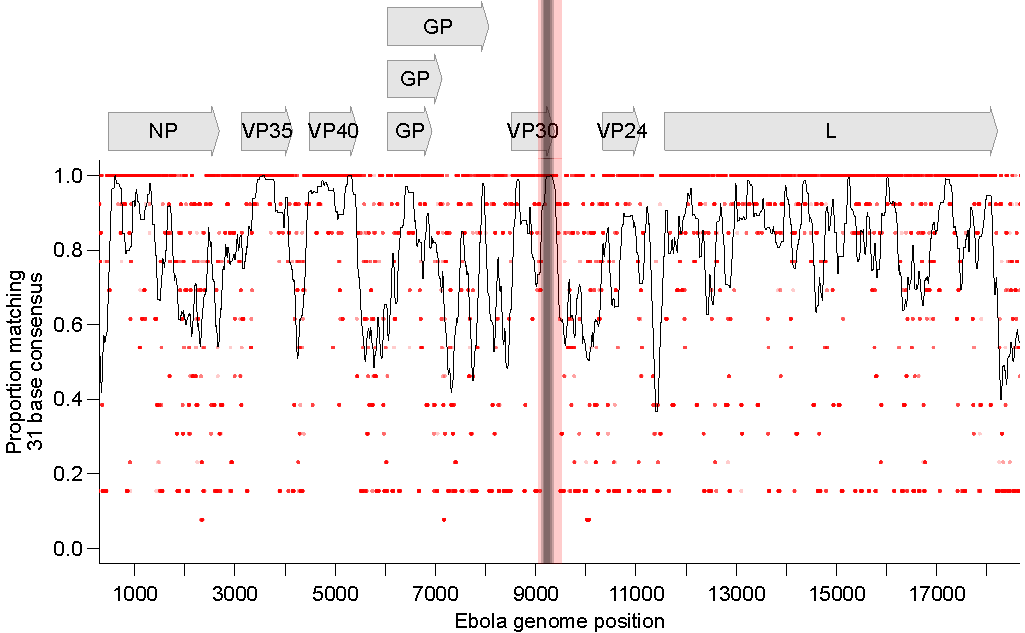
\includegraphics[width=.6\textwidth]{ebolaConsensus.pdf} %REMOVE%
		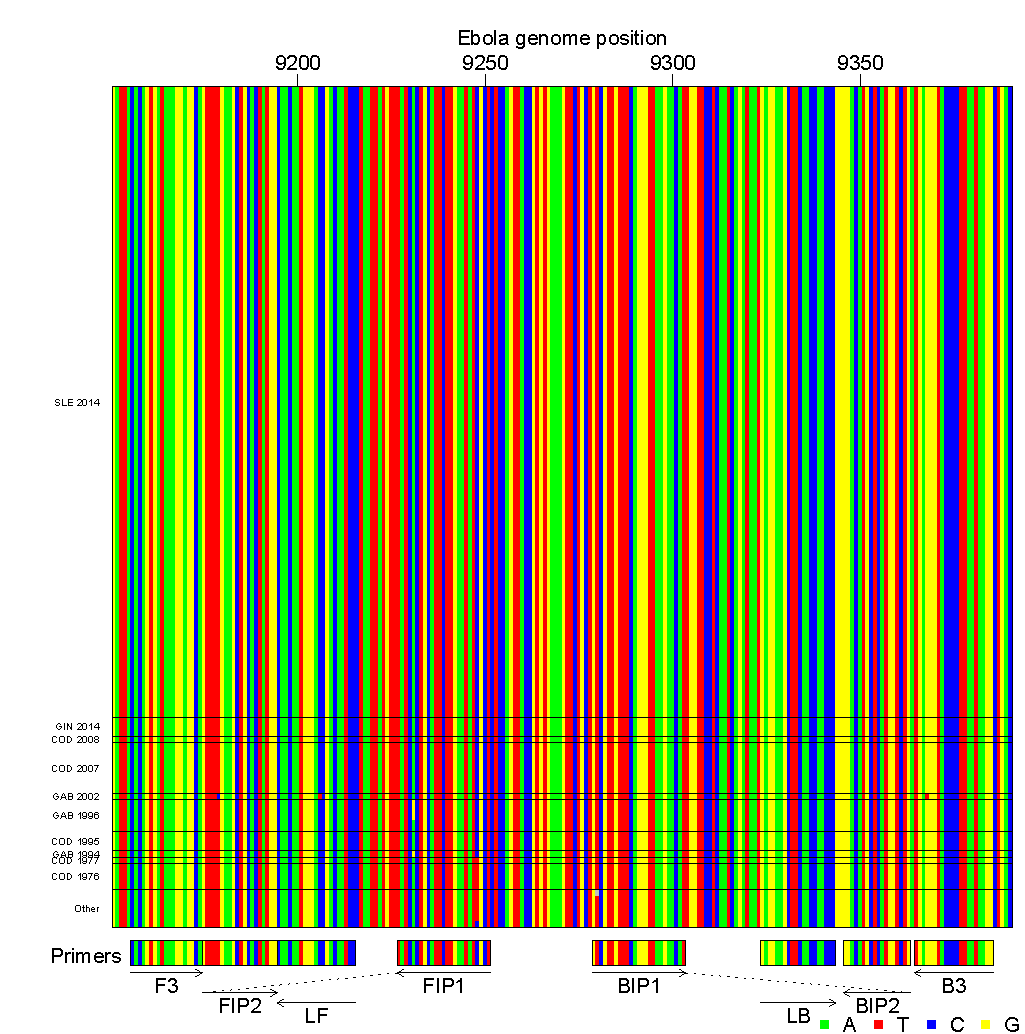
\includegraphics[width=.6\textwidth]{loop_bases.pdf} %REMOVE%
		\caption[Ebola RT-LAMP primers design]{Bioinformatic analysis to design Ebola RT-LAMP primers. A) Conservation of sequence in Ebola. Ebola genomes (n = 131) from Genbank and sequences from the recent Zaire Ebolavirus outbreak \citep{Gire2014} were aligned and conservation calculated. The x-axis shows the coordinate on the Ebola genome, the y-axis shows the proportion of sequences matching the consensus for each 21 base segment of the genome (red points). The black line shows a 101 base sliding average over these proportions. The vertical red shading shows the region targeted for LAMP primer design that was used as input into the EIKEN primer design tool. Numbering is relative to the Ebola Mayinga sequence. B) Aligned genomes, showing the locations of the preliminary primers. Sequences in the red shaded region in A are shown, with DNA bases color-coded as shown at the lower right. Each row indicates an HIV sequence and each column a base in that sequence. Horizontal lines separate Ebolavirus outbreaks (labeled at left). Arrows indicate the strand targeted by each primer. Primers targeting the negative strand of the virus are shown as reverse compliments for ease of viewing.}
		\label{figEbolaConsensus}
	\end{figure}

\subsection{Conclusions}
	These studies contribute the study and treatment of HIV-1 by revealing aspects of latency, expression and host response. They highlight the importance of primary cell models and the effects that host cell can have on viral processes. With rapidly increasing sequencing throughput, studies like those presented in this thesis offer the opportunity for a deeper and broader understanding of HIV-1 biology and host response and further development of diagnostics and therapeutics.

\end{document}
